% begin module tangent-line-polynomial
\begin{frame}
\begin{example}[Tangent Line on a Polynomial]
Find an equation for the tangent line to the parabola $y = x^2 +2x + 1$ at the point $P = (2,9)$.

\begin{columns}[c]
\column{.4\textwidth}
\ \uncover<2->{%
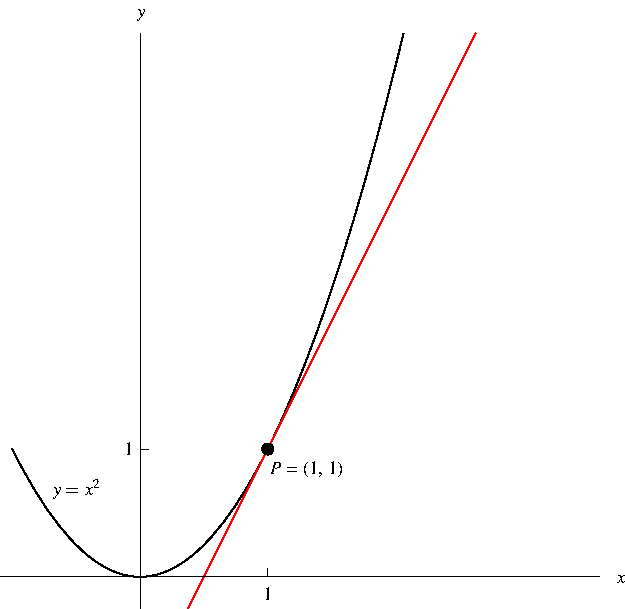
\includegraphics[height=4.5cm]{derivatives/pictures/02-01-secanta.pdf}%
}%
\column{.6\textwidth}
\uncover<2->{%
Here $a = 2$ and $f(x) = x^2 + 2x +1$.
}%
\abovedisplayskip=0pt
\belowdisplayskip=0pt
\abovedisplayshortskip=0pt
\belowdisplayshortskip=0pt
\begin{align*}
\uncover<3->{m} & \uncover<3->{ = }  \uncover<3->{\lim_{x\rightarrow 2} \frac{f(x)-f(2)}{x-2}}\\
& \uncover<4->{ = }  %
\uncover<4->{\lim_{x\rightarrow 2}\frac{x^2+2x - 8}{x-2}}\\
& \uncover<5->{ = }  %
\uncover<5->{\lim_{x\rightarrow 2}\frac{(x - 2)(x+4)}{x-2}}\\
& \uncover<6->{ = }  %
\uncover<6->{\lim_{x\rightarrow 2} x+4 }\\
& \uncover<7->{=} %
\uncover<7->{6 }
\end{align*}
\uncover<8->{
Point-slope form: $y - 9 = 6(x - 2)$, or $y = 6x - 3$.
}
\end{columns}
\end{example}
\end{frame}
% end module tangent-line-polynomial
